\documentclass[a4paper]{jpconf}
\usepackage[utf8]{inputenc}
\usepackage{graphicx}
\usepackage{lmodern}
\bibliographystyle{iopart-num}


\begin{document}
\title{The Neutron Monitor Control Panel}

\author{O García-Población$^{1,2}$, H Ivanov$^2$, I García-Tejedor$^{1,2}$,
J J Blanco$^{1,2}$, J Medina$^{1,2}$, R Gómez-Herrero$^{1,2}$, E
Catalán$^{1,2}$ and D Radchenko$^{2}$}

\address{$^1$ Space Research Group, University of Alcalá, Spain}
\address{$^2$ Castilla-La Mancha Neutron Monitor, Parque Tecnológico de Guadalajara, Spain}

\ead{oscar.gpoblacion@uah.es}

\begin{abstract} 

    This work presents the current status and future plans of the Neutron
    Monitor Control Panel (NMCP), a new software developed to aid the operator
    in typical station maintenance and configuration operations. This software
    is integrated with the new so called NOAS data acquisition system and it
    can be accessed using a supported web browser. It features a visual
    inspection tool to help the operator to identify spikes in the data, trace
    the origin of the spike back to the raw readings of each counter tube and
    pressure reading, and mark the data as invalid in the Neutron Monitor
    Database if desired. The software also provides information about station
    operation status, some descriptive statistics about current data being
    recorded and, in the future, will provide an interface to configure station
    parameters.

\end{abstract}

\section{Introduction}

Neutron Monitor data are widely used by researchers in different research
fields not necessarily related to cosmic rays, such as space weather and/or
geomagnetic studies. That's why the Neutron Monitor Database
(NMDB)\cite{NMDB2011} puts effort into delivering data with the best quality
possible. The data are also used in real-time GLE alarm systems and other
real-time applications; therefore, the data quality protocol must be applied in
real-time. Eventually, the data will be revised by a human supervisor to ensure
the correct behaviour of the quality protocol. By quality protocol we refer to
all the methods and techniques used such as:

\begin{itemize}
	\item Detection of abnormal data, commonly referred to as spikes.
    \item Detection of inactivity, i.e, there are no data uploaded in NMDB for
        the last minutes. This will lead to a notification to the team
        responsible for the Neutron Monitor station. 
    \item Neutron monitors are formed by several counter tubes, typically
        eighteen. A malfunction in a single tube shouldn't make the entire
        station stop reading cosmic rays measurements. While it is true that
        missing counters degrades the quality of the measurement by increasing its
        variability, if the number of working tubes is enough the result can
        still be acceptable. This leads us to the need of monitoring and
        detection of malfunctions separately in each of the tubes.  
    \item Detection of changes with respect to the historical activity.
        Since changes in the immediate environment or the instruments can cause
        overall changes in the measured values of a Neutron Monitor, detecting
        and correcting those changes is desirable.
    \item Comparing the data from one station to the data of different nearby
        stations. Detecting isolated events could indicate that there is a
        malfunction in that station.	
\end{itemize}

Once the corrupted data are detected, the cause of such data corruption can
often be traced down to its cause. Most of the times those malfunctions are
caused by the instruments forming the data acquisition system, so detecting the
corrupt data and its cause helps us improve and learn more about it. The figure
\ref{fig:NoisePoints} shows schematically the main sources of errors. Most of
them are Electro-Magnetic Interferences (EMI) in the preamplifiers (A), in the
transmission lines from the amplifiers to the data acquisition system (B) and in
the data acquisition hardware itself (C). Also malfunctions in the software (D)
can introduce undesirable artifacts in the data.

\begin{figure}[ht]
    \centering
    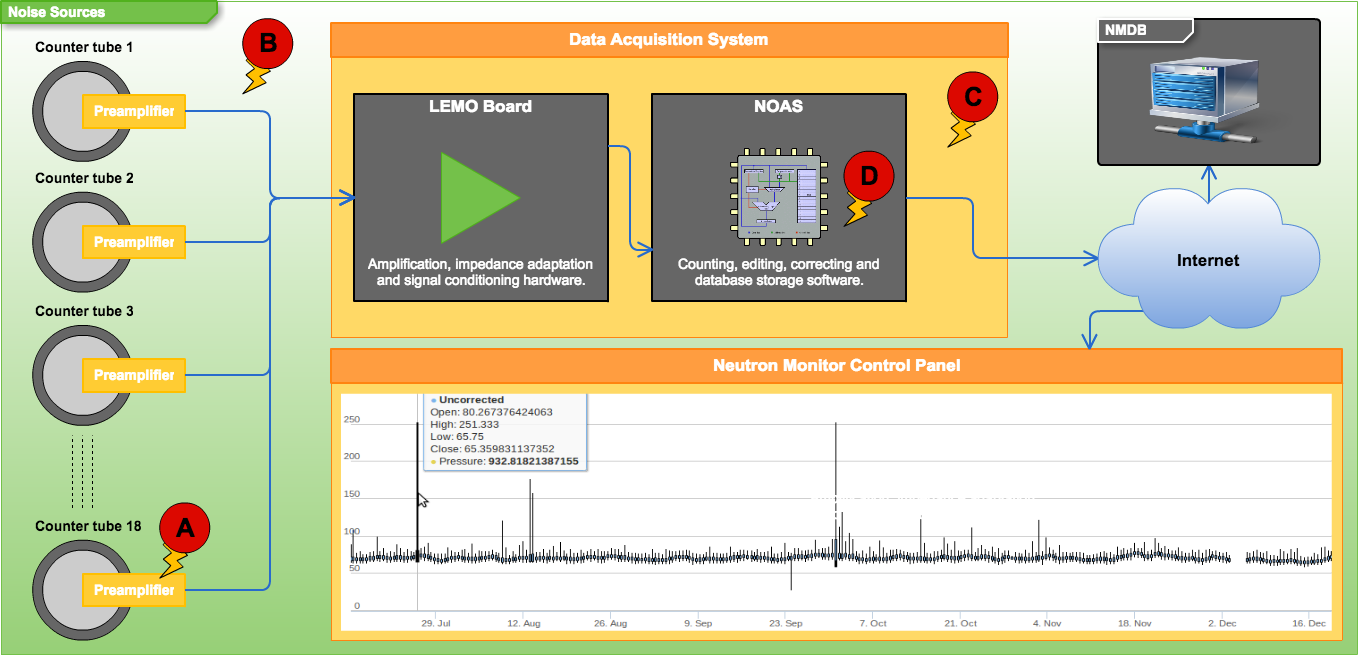
\includegraphics[keepaspectratio, width=1\textwidth]{./resources/NoisePoints.png}
    \caption{Possible error sources.}
    \label{fig:NoisePoints}
\end{figure}

In order to ease the detection of the corrupt data we are working in the
development of a Web tool which will help us detect these corruptions. The Web
application makes use of dynamically generated plots which are designed to
highlight possible corrupted data.

This software is currently running for testing in the second release of the data
acquisition system\cite{Garcia2014} designed for the CaLMa\cite{Medina2013} and
KIEL2 stations.


\section{System architecture}

There are two main elements in the architecture: a client that requests and
consumes data using a web browser, and a system that collects and serves the
data, which in this system is the data acquisition system. This separation of
roles follows the client-server design pattern\cite{wiki:ClientServer}.The
figure \ref{fig:arch} shows a block diagram with all the components involved
along with its relationships. Each block and relationship will be described
bellow.

The software architecture is based on the Model-View-Controller (MVC) software
design pattern\cite{wiki:MVC}. This pattern encourages the separation between
the data, the data processing and the data representation. 

The view component is in charge of the data representation and the user
interface. In our system, this component is mainly executed by the client in a
web browser, which is not only a convenient graphical output device but also
provides a way to interact with the user. In response to these interactions, the
browser makes requests to a server which answers back with new data to be
represented. All the software running in this component has been written in
JavaScript, and makes intensive use of two libraries:
HighStock\cite{web:highstock} to draw plots and charts, and Sencha
ExtJS\cite{web:extjs} which is a very powerful framework that handles between
other things the graphical user interface.

The model component is located on the server side, in the data acquisition
system. This model comprises all the data captured from each counter tube and
the algorithms used to process these data, such as atmospheric pressure
corrections, sanity checks, editors to combine all the readings into a single
one, etc. There are two databases involved in this component, one in the data
acquisition system itself and another in a regular server. The first one is a
small and light SQLite database, running in the data acquisition system on a
Beagle Bone Black embedded system\cite{Garcia2014}. This database stores per
detector count rates, atmospheric pressure and voltage levels along with a time
stamp. The data from this database are edited, corrected and sent to a second
database server running MySQL\cite{web:mysql}. This is an enterprise grade
relational database server, used also by NMDB. The software needed to implement
the editors, corrections, and transfer between databases has been written in PHP
programming language, using the Zend\cite{web:zend} as support framework.

Several controllers adapt and serve the model data as REST-like web services,
using JSON\cite{wiki:JSON} for data representation. REST is a well known
software architecture that constraints the design of components to increase
compatibility and isolation, standardising the way that services can be
consumed. This web services are designed to be a documented Application
Programming Interface (API) for accessing the station information and services,
allowing third party applications to be further developed. The main consumer of
this API right now is the spike tool, which is used to track and mark anomalous
surges in the data from the station. The next section describes this tool in
detail.

\begin{figure}[h]
    \centering
    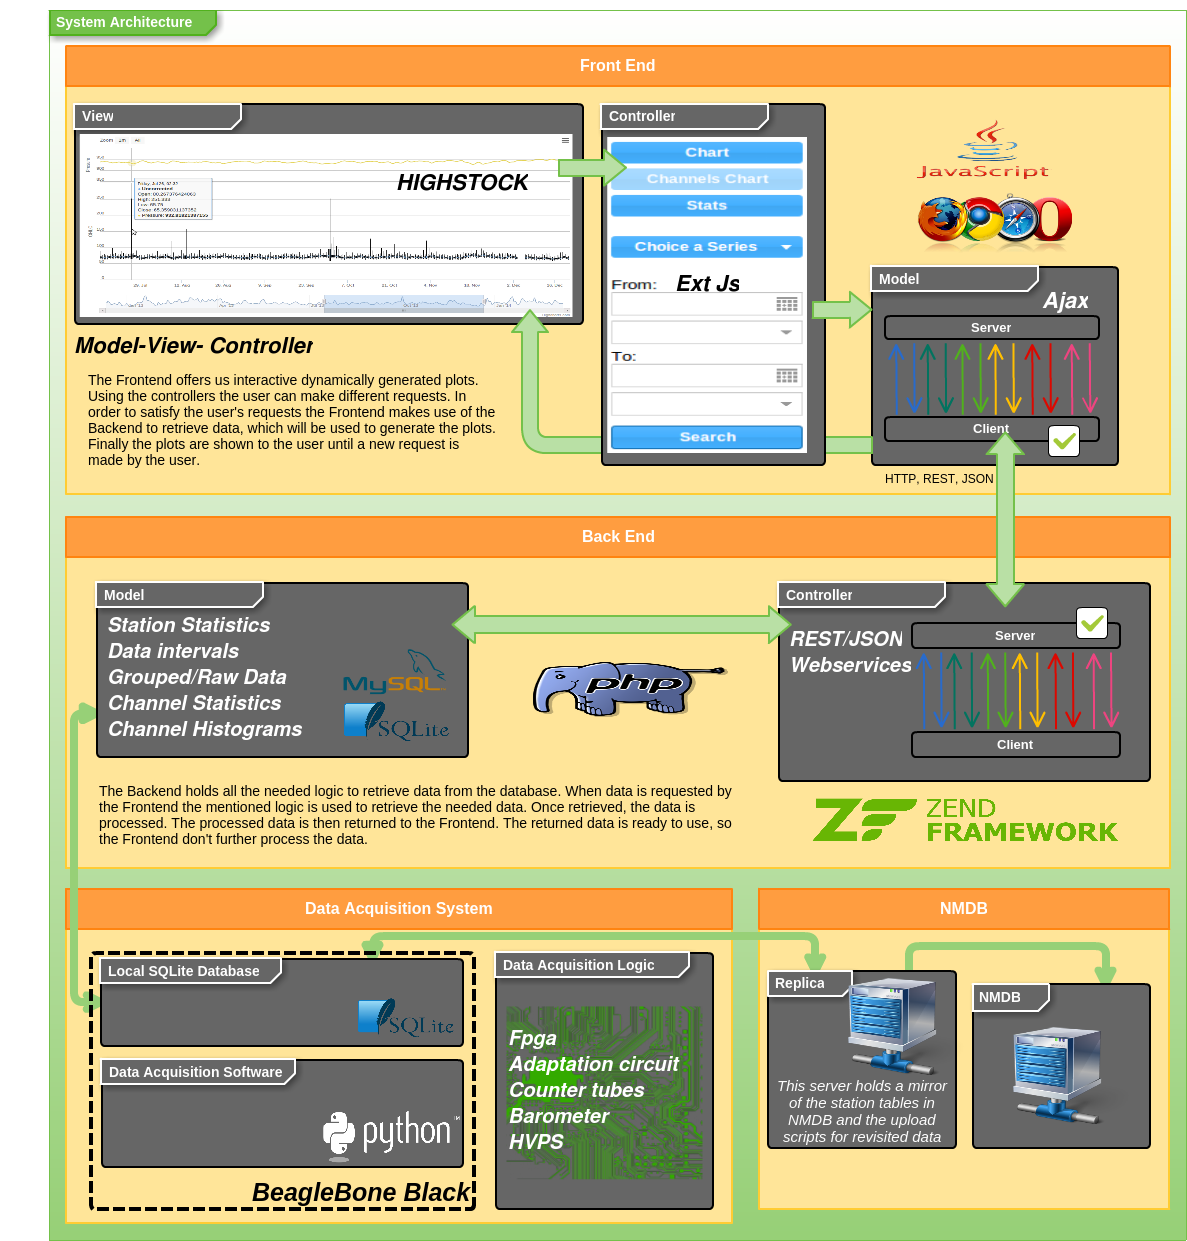
\includegraphics[keepaspectratio, width=1\textwidth]{./resources/Architecture.png}
    \caption{System architecture}
    \label{fig:arch}
\end{figure}

\section{The spike tool}

Currently the Spike Tool consists of three modules, \texttt{Spike},
\texttt{SpikeCorrected} and \texttt{ChannelStats}. \texttt{Spike} and
\texttt{SpikeCorrected} are very similar, but \texttt{SpikeCorrected} works with
a different set of data and has some extra functionality.

The \texttt{Spike} module offers an interactive chart in which the spikes
are easy to trace. As shown in the figure \ref{fig:SpikeTool}, initially the
chart displays a large set of data, and some kind of data grouping is needed.
Just averaging the data flattens the spikes.  The Candlestick chart is used to
prevent the aforementioned problem, as this way the max and min values can be
easily distinguished. Eventually when a short interval of data is requested and
no grouping is needed to display it, the chart will automatically switch to a
line chart.

As mentioned above the chart is interactive, and offers a very intuitive
zooming functionality. Clicking and dragging through an interval of the chart will
raise a zoom event, and depending on the drag direction the event will be zoomed In
or Out. The chart also offers a navigator which allows us to navigate forwards or
backwards in time. Datetime input fields are available too, which allows the user to
plot a specific time interval.

At first the uncorrected data are used to generate the charts, but we are given
the chance to choose between Uncorrected data and Efficiency and Pressure corrected
data. The atmospheric pressure is also plotted, which helps us to evaluate how the
atmospheric pressure affects the measurements of our Neutron Monitor station.

Once we have a spike located, we can see the raw reading of the counter tubes,
which allows us to better track the spike. Due to the fact that there are 18
channels this option is available only when no data grouping is needed.

As said before, the \texttt{SpikeCorrected} module is very similar to the
\texttt{Spike} module which was explained above. First of all, this module makes
use of a different set of data. The \texttt{Spike} module uses the raw data which
comes from the data acquisition system while \texttt{SpikeCorr} uses the
revised data, and also provides the ability to update the revised data.

Clicking on a value in the chart will mark the clicked data, which is
stored in a table. The data in the table can be later submitted to the revised
set of data, which means that the mentioned data will be considered invalid and
treated as void in the future.

The table which contains the marked data can be seen on a separate window, which
can be show and hidden when needed. The window also contains all the
controls needed for submitting and unmarking the marked data.

The last module, \texttt{ChannelStats}, is intended to give information about the
different channels separately, so that we can identify malfunctions on isolated
channels. The module offers various statistics for user defined time intervals,
among which the simplest are the average value, minimum/maximum
values and standard deviation.

The \texttt{ChannelStats} module offers distribution charts, too. Histograms with the
channels' raw data are plotted in the requested time intervals. The chart is
highly interactive, and the series can be shown, hidden and highlighted. Currently
we are working on this module.

\begin{figure}[h]
    \centering
    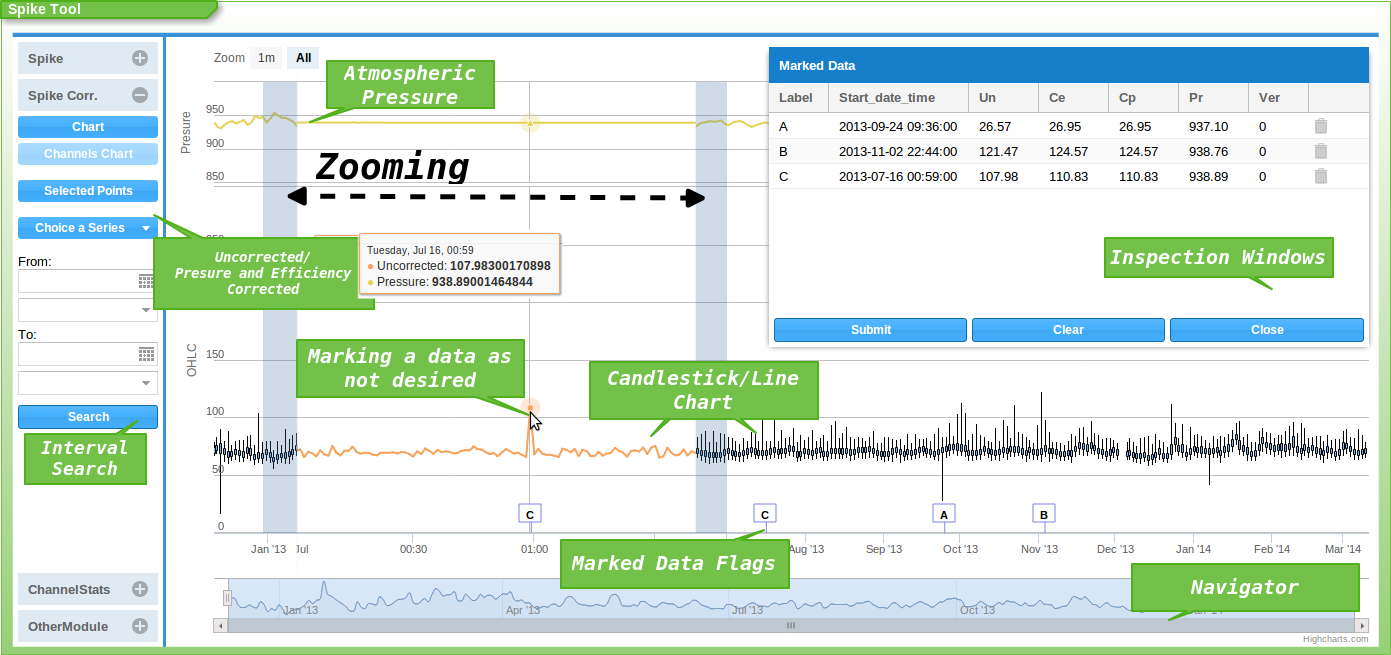
\includegraphics[keepaspectratio, width=1\textwidth]{./resources/SpikeTool.png}
    \caption{Spike Tool}
    \label{fig:SpikeTool}
\end{figure}

\section{Future work}

The Neutron Monitor control panel is a natural add-on to the new data
acquisition system designed for Neutron Monitors and is under active
development to add new useful features in the near future. Some of these future
features are summarized below.

\begin{description}
    \item[Online statistics] The control panel will include a module for
        descriptive statistics that will be calculated in real-time from the
        counter tubes raw readings. This will help to identify drifts in the
        behavior of the detectors and to apply the appropriate actions to
        maintain data quality.
    \item[Station reconfiguration] This will allow the operator to disconnect a
        counter from the station without affecting global station count. This
        can be useful to perform maintenance operations such as counter tube
        diagnostics. 
    \item[Station parameter setup] New electronics allow the remote control of
        some parameters, for example the high voltage power supply set point,
        the remote database for data upload, backup policies, etc.
    \item[Alarms and push notifications] When connectivity allows it, it will
        be possible to configure alarms and notifications to recipients using
        the new push mobile technologies. For example, if the station is no
        longer uploading data to NMDB or if its data is out of quality
        standards
    \item[Detector response histogram] A new design from University of New
        Hampshire of the front-end amplifiers provides a pulse which width is
        proportional to the energy of the incident particle. The new data
        acquisition system NOAS features a different programmed core running in
        its Field Programmable Gate Array (FPGA) device. This core enables the
        system to read these pulses and to generate a histogram with the
        distribution of the pulse energy over a given time interval. This will
        enable a mechanism for non-intrusive diagnostics of the counter tubes.
        This means that diagnostics can be carried out without disconnecting the
        detector, changing its biasing voltage or, in general, altering its
        normal operational parameters. Therefore there is no need to interrupt
        the radiation measurements while the tests are being conducted.
\end{description}

Even though this tool is focused on spikes, there are many other data anomalies
that affect data quality, like data drifts, steps, missing data, and so on.
Dealing with each one of these requires a very different approach and further
study is therefore required. When available, the software designed to address
these problems could be easily integrated in the NMCP as a new service.

\subsection*{Acknowledgments} 

The authors would like to thank the Guadalajara Science and Technology Park for
its support for this project.


\section*{References}
\bibliography{iopart-num} 

\end{document}


